\chapter{Introduction}
\pagenumbering{arabic}

\section{\acl{adas}}
\label{sec:adas}
Advanced Driver Assistance Systems (ADAS) are technologies that improve road 
safety by enhancing both vehicle and driver capabilities. These systems support 
the driver in the driving process, reducing the likelihood of human error and 
increasing road safety. ADAS includes a range of features from basic functions 
such as automatic headlights and rain-sensing windshield wipers to more complex 
systems like adaptive cruise control, lane departure warning, and collision 
avoidance systems.

The evolution of ADAS has been fueled by advancements in sensors, computing 
power, and connectivity. These technologies work together to provide vehicles 
with the ability to not only sense their environment but also to analyze and 
respond to potential hazards. As such, ADAS is seen as a crucial step towards 
fully autonomous vehicles, providing a safer, more comfortable driving experience.

\subsection{Market Size and Growth}
The market for \ac{adas} is experiencing robust growth as these technologies 
become more integral to new vehicle designs, emphasizing safety and driving 
efficiency. 

In 2024, the global ADAS market is projected to be worth around 
\$64.05 billion, with expectations to expand significantly at a \ac{cagr} 
of 12.7\% reaching approximately \$211.71 billion by 2034 \cite{adas_report_2023}.
This growth is given by advancements in autonomous driving technology and 
an increasing emphasis on vehicle safety from both consumers and functional 
safety certifications. 
Significant investments are also being made in the development and 
implementation of ADAS technologies across various global markets, including 
Japan, China, the United States, and Europe \cite{adas_report_2023}.

\begin{table}[h]
    \centering
    \begin{tabular}{r|c}
        \hline
        \textbf{Market} & \textbf{CAGR} \\
        \hline
        Worldwide & 12.7\% \\
        Japan & 13.6\% \\
        China & 13.5\% \\
        United States & 12.5\% \\
        Canada & 9.7\% \\
        Germany & 8.8\% \\
        Spain & 8.5\% \\
        \hline
    \end{tabular}
    \caption[CAGR of the ADAS market in different countries]
    {\ac{cagr} of the ADAS market in different countries \cite{adas_report_2023}.}
    \label{tab:adas_revenue}
\end{table}
Considering the market value and growth rate of \ac{adas} technologies, 
ADAS systems must also be economically viable on a large scale. 
This necessitates the use of cost-effective sensors such as cameras and radars, 
which offer a balance between performance and affordability. While there are 
more accurate options available, such as LiDAR sensors, these are typically more 
expensive and are primarily used for self-driving car experiments in research 
laboratories. The high cost of LiDAR sensors makes them less suitable for 
widespread deployment in consumer vehicles. Therefore, the challenge lies in 
leveraging affordable technologies like cameras and radars to their maximum 
potential, to deliver effective ADAS systems that can be widely adopted.

\subsection{Market Ecosystem}
The market ecosystem for \ac{adas} can be 
conceptually divided into several layers, each representing a different segment 
of the value chain. These layers range from \acp*{oem} to the suppliers of the key 
components such as sensors and processors. 
Here's a breakdown of these layers and the main companies in each field:

\subsubsection*{\acp{oem}}
\aclp{oem} are companies that integrate ADAS into their vehicles. They either develop 
some of their own ADAS technologies or incorporate systems designed by 
Tier 1 suppliers. Some of the leading \acsp{oem} in the ADAS market include 
Honda, Toyota, Nissan, General Motors, Tesla, Ford, Volkswagen, Volvo, BMW, and 
Mercedes-Benz.

\subsubsection*{Tier 1 Suppliers}
Tier 1 suppliers develop complete systems or significant components that are 
directly supplied to \acp{oem}. These companies often develop the software and 
hardware integration necessary for ADAS.
Main Tier 1 suppliers in the ADAS market include Bosch, Continental, Aptiv, 
Denso, Magna, and Valeo.

\subsubsection*{Autonomous Technology Developers}
This layer includes companies specifically focused on developing software and 
platforms that enable autonomous driving capabilities beyond standard ADAS features.
Key players in this segment include Waymo (Google/Alphabet), Cruise (General Motors),
Argo AI (Ford, Volkswagen), Aurora, and Zoox (Amazon).

\subsubsection*{Sensing and Perception}
Companies in this segment focus on developing sensors and perception technologies 
that allow vehicles to perceive their environment, which is essential for both 
ADAS and fully autonomous functionalities.
Main providers are Luminar (LiDARs), Velodyne (LiDARs), Mobileye (cameras), 
Foresight Autonomous (cameras).

\subsubsection*{Processors and Computing}
This segment involves the manufacturers of the advanced computing systems that 
process inputs from various sensors to make real-time driving decisions.
Key players include NVIDIA (GPUs and SoCs), Intel (through Mobileye), 
Qualcomm (processors), NXP Semiconductors (microcontrollers), and 
Renesas (microcontrollers and SoCs).

\subsubsection*{Sensors}
This layer includes manufacturers of the various types of sensors used in ADAS 
and autonomous vehicles, such as cameras, radar, LiDAR, and ultrasonic sensors.
Main companies in this segment include Bosch (radar and video sensors),
Continental (radar sensors), Sony (image sensors), Texas Instruments (radar chips),
and ON Semiconductor (image sensors for automotive cameras).


\subsection{Key Components of \acs{adas}}
\ac{adas} systems are composed of several key components that work together to 
enhance vehicle safety and driving experience. These components include sensors, 
control units, actuators, human-machine interface, and connectivity.
\begin{figure}
    \centering
    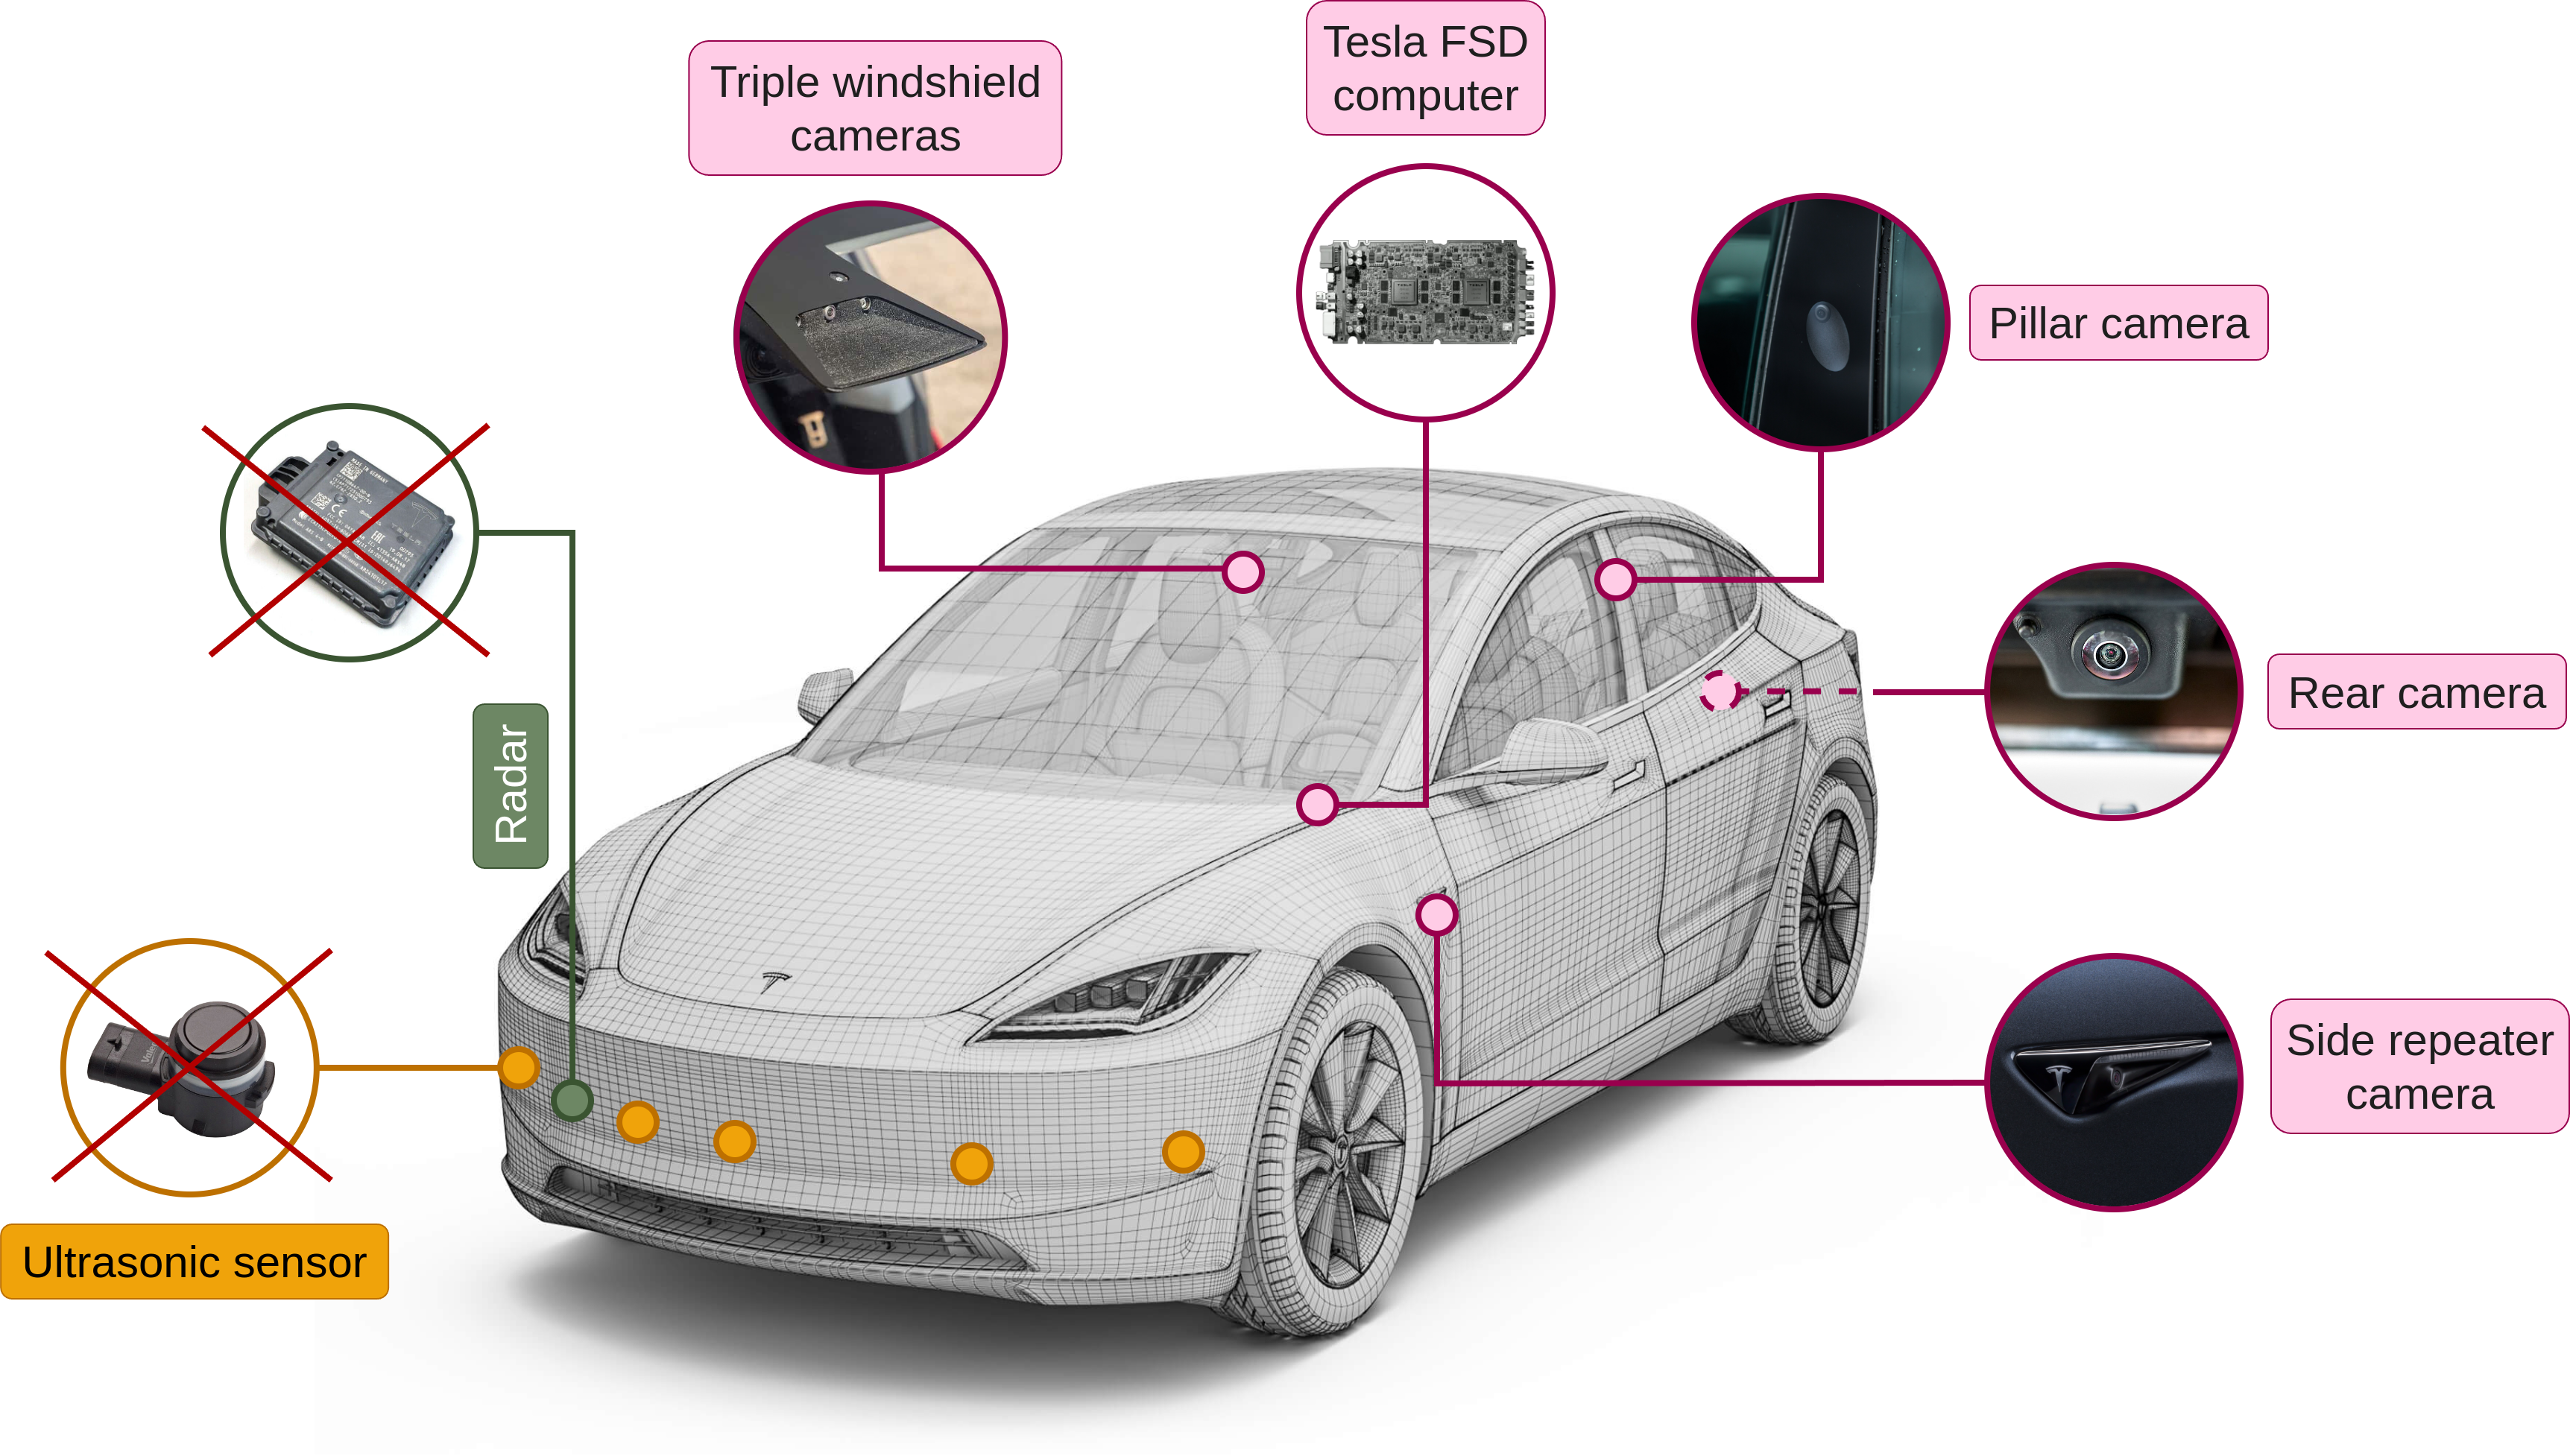
\includegraphics[width=\textwidth]{images/introduction/tesla_sensors.png}
    \caption[Components of an ADAS system]
    {\acs{adas} sensors in a 2024 Tesla Model 3. Modified image source: 
    \cite{mantangcg_2024_tesla_model_3}.}
    \label{fig:adas_components}
\end{figure}

\subsubsection*{Sensors}
Sensors help the vehicle perceive its environment by collecting data on the 
surrounding objects and road conditions. The main types of sensors used in ADAS 
systems are:

\begin{itemize}
    \item \textbf{Radar Sensors}: These sensors use radio waves to detect the 
    distance and speed of objects around the vehicle. They are particularly 
    useful for measuring the relative speed of other vehicles and detecting 
    objects in poor weather conditions.
    
    \item \textbf{Cameras}: Cameras provide visual data that is used for object 
    recognition, lane detection, traffic sign recognition, and other visual 
    tasks. They are essential for understanding the vehicle's surroundings and 
    identifying potential hazards.
    
    \item \textbf{Ultrasonic Sensors}: These sensors are used for close-range 
    detection, primarily in parking assistance systems. They help the vehicle 
    detect obstacles when maneuvering at low speeds.
    
    \item \textbf{LiDAR}: LiDAR sensors use laser pulses to create a 3D map of 
    the vehicle's surroundings. They are particularly useful for creating 
    detailed maps of the environment and detecting objects at longer ranges.
\end{itemize}

\subsubsection*{Control Units}
Control units are responsible for processing the data from sensors and cameras, 
making real-time decisions, and sending commands to the vehicle's actuators.
Decision making algorithms are implemented in these units to interpret sensor 
data and determine the appropriate response to different driving scenarios.

\subsubsection*{Actuators}
Actuators are the components that control the vehicle's braking, steering, and 
acceleration systems based on the commands received from the control units. 
These actuators are responsible for executing the decisions made by the ADAS 
to ensure safe and efficient driving.

\subsubsection*{Human-Machine Interface}
The human-machine interface is the system through which the driver interacts 
with the ADAS. This interface includes displays, alerts, and notifications that 
inform the driver about the status of the vehicle and provide warnings or 
assistance when needed. The interface is crucial for ensuring that the driver 
remains aware of the vehicle's behavior and can intervene when necessary.

\subsubsection*{Connectivity}
Connectivity is an essential component of modern ADAS systems, enabling 
communication between the vehicle and external systems. This connectivity allows 
the vehicle to receive real-time traffic information, software updates, and 
remote assistance. It also enables vehicle-to-vehicle and vehicle-to-infrastructure 
communication, which is crucial for advanced safety features like collision 
avoidance and traffic management.


\subsection{Common \acs{adas} Features}
ADAS systems offer a wide range of features that enhance vehicle safety, 
comfort, and efficiency. Some of the most common ADAS features include: 
\ac*{acc}, \ac*{ldw}, \ac*{bsd}, \ac*{aeb}, \ac*{tsr}, \ac*{dms}, parking assistance,
adaptive headlights, and more. Most important functionalities are described in detail.

\subsubsection*{\ac{acc}}
\ac{acc} is a feature that maintains a set speed and adjusts it to keep a safe 
distance from the vehicle ahead. It uses sensors to detect the distance and 
speed of the vehicle in front and automatically adjusts the vehicle's speed to
maintain a safe following distance.

\subsubsection*{\ac{ldw}}
\ac{ldw} is a system that alerts the driver if the vehicle begins to drift out 
of its lane without signaling. It uses cameras or sensors to monitor the vehicle's 
position within the lane and provides visual or audible warnings if the vehicle 
starts to veer off course. Some vehicles also have \ac{lka} systems that can 
automatically steer the vehicle back into its lane if the driver does not respond 
to the warnings.

\subsubsection*{\ac{bsd}}
\ac{bsd} is a system that warns the driver of vehicles in the blind spot during
lane changes. It uses sensors to detect vehicles in adjacent lanes that may not
be visible in the side mirrors and provides visual or audible alerts to prevent
collisions during lane changes.

\subsubsection*{\ac{aeb}}
\ac{aeb} is a safety feature that detects imminent collisions with vehicles,
pedestrians, or other obstacles and automatically applies the brakes to prevent
or mitigate the impact. This system helps reduce the severity of accidents by
providing an additional layer of protection when the driver fails to react in
time.

\subsubsection*{\ac{tsr}}
\ac{tsr} is a feature that uses cameras or sensors to identify traffic signs
such as speed limits, stop signs, and road markings. It displays this information
on the vehicle's dashboard or head-up display, helping the driver stay informed
about the current road conditions and regulations.

\subsubsection*{\ac{dms}}
\ac{dms} is a system that monitors the driver's attention and alertness while
driving. It uses sensors to track the driver's eye movements, head position, and
other behavioral cues to detect signs of drowsiness, distraction, or inattention.
The system can provide warnings or take corrective actions to prevent accidents
caused by driver fatigue or distraction.
%
\section{Focus of this work}
\label{sec:focus}
This thesis delves deep into the development of a computer vision-based system 
to warn drivers about potential hazards on the road. The first part is more 
focused on monitoring the driver's behavior and attention through its gaze, and 
outside-world interactions with vulnerable road users. During this phase, 
an initial scheme to analyze the driver's gaze and its interaction with the 
environment is proposed. In particular, the model is based on extracting indirect 
features from sensors, location of vulnerable users during the time, projection 
of the driver's gaze to the scene, and estimation of the depth of the scene.
However, we also highlight the limitations of this approach, mainly due to the 
complexity of the task, and the unreliability of some algorithms used for 
extracting features from the scene.

In the second part, we move to a deep learning-based approach to solve the 
problem of detecting potential hazards on the road. The idea is to have a model 
that can approximate human-like decision making adding some biases to the 
training data.
We focus on training a model 
able to capture the spatial information of the scene, and to predict the presence 
of anomalies in the driving environment. We also explore the possibility of 
leveraging the large quantity of unlabelled data to increase the performance 
of predictions through semi-supervised learning techniques.
At the end, we also explore the potential of few-shots learning with large 
pre-trained models, making some experiments with GPT-4o. This is to demonstrate 
how the model's architecture is suitable for the required tasks with enough 
prior knowledge. It is also interesting to see how the model can adapt to 
the specific domain without changing its parameters and only thanks to the 
attention mechanism.

In the second part we also deeply discuss the training pipeline, which consists 
of data selection and pre-processing, model architecture, and evaluation metrics.
In particular, we analyze how common evaluation metrics can be misleading 
when dealing with unbalanced datasets, and how \ac{roc} and \ac{auc} are 
more reliable metrics for evaluating the performance of the model.
Therefore, we also provide a training method to deal with this type of datasets,
that are prevalent in the field of anomaly detection in driving scenarios.

Another contribution is the discussion of possible future works, 
depending on the results obtained from the experiments and the limitations 
encountered during the development of the project.


\section{Thesis Organization}
\label{sec:organization}
The remainder of this thesis is organized as follows: 
\begin{itemize}
    \item \textbf{Chapter \ref{chpt:related_work}} provides an overview of the 
    state-of-the-art methods and models for object tracking, image and video 
    classification. It discusses how model complexities and relative computational 
    costs increased in the last decade, comparing their performance on benchmark 
    datasets. It also compares available datasets containing driving scenarios 
    for different tasks. Finally, it goes deep into existing model architectures 
    and datasets for anomaly detection in driving scenarios, which is closely 
    connected to our work.
    \item \textbf{Chapter \ref{chpt:background}} presents main algorithms and 
    architectures used for developing the project. It is mainly divided into 
    two sections: traditional computer vision and deep learning-based techniques.
    The former includes explanations of the SIFT algorithm \cite{lowe_sift} and 
    estimation of the homography matrix. The latter includes the Meta Pseudo-Labels 
    algorithm \cite{pham2021meta} and the vision transformer architecture \cite{vit},
    with a focus on all stages involving the multi-head self-attention mechanism.
    \item \textbf{Chapter \ref{chpt:methods}} describes all the methodologies 
    and hypothesis for making the experiments; it is also divided in traditional 
    computer vision and deep learning-based techniques.
    The former includes a general scheme of the driver's attention model, 
    a description of how data is structured and processed, a brief comparison of 
    possible methodologies for estimating the depth, and an explanation of how 
    introducing spatial information of scenes is beneficial.
    The latter includes a general scheme for representing the task to be solved, 
    the training pipeline for making experiments with the DR(eye)VE dataset, and 
    data pre-processing for both DR(eye)VE \cite{dreyeve} and BDD-100K 
    \cite{bdd100k} datasets. 
    \item \textbf{Chapter \ref{chpt:experiments}} shows results obtained from 
    the experiments made with the traditional computer vision and deep learning 
    approaches. For the former case, it includes projection of the gaze, 
    data distribution of the DR(eye)VE dataset, interaction between the 
    driver's gaze and vulnerable road users, accuracy of the monocular depth 
    estimation of MiDaS \cite{midas}, and tracking errors with ByteTrack \cite{bytetrack}. 
    It also discusses limitations of this method 
    and motivations for moving to deep learning-based techniques.
    For the latter case, there are experiments comparing supervised and 
    semi-supervised learning on the DR(eye)VE and BDD-100K dataset. There is also 
    a further experiment on few-shots inference of the GPT-4o model with the 
    BDD-100K dataset, to demonstrate potential performances of task-related 
    knowledge distillation from pre-trained large models to smaller ones
    \cite{yu_knowledge_distillation}.

    \item \textbf{Chapter \ref{chpt:conclusion}} concludes the thesis by summarizing 
    the key contributions, discussing possible problems and limitations that 
    affected the experiments, and outlining potential directions for future work.
    There is also a consideration of how driver's gaze data can be combined with 
    deep learning-based techniques to warn the driver about potential hazards, 
    considering realtime constraints and the need for a reliable system.
    \item \textbf{Appendix \ref{appendix:training_algorithms}} lists main custom 
    algorithms used for the experiments, including data pre-processing and the 
    training pipeline for updating the quantity of labelled samples in the DR(eye)VE dataset.
    \item \textbf{Appendix \ref{appendix:auc_probabilistic}} provides a more 
    formal and detailed explanation of the \acs{auc}-\acs{roc} from a probabilistic
    perspective. It is an helpful appendix to better interpret results on 
    experiments with unbalanced datasets and to understand strenghts and 
    limitations of available evaluation metrics.
\end{itemize}
